\documentclass[preprint]{ccn}
\addbibresource{ccn_references.bib}

% Author comment commands
\newcommand{\TS}[1]{\textcolor{magenta}{[\textbf{TS:} #1]}}

\title{Harmonizing the TIMM Model Zoo with Human Visual Strategies}

\author{Author1, Author2, Author3, Author4 \\
  Department of Cognitive and Psychological Sciences, Brown University \\
  \email{example@brown.edu}}


\begin{document}

\maketitle

\TS{We need a better name than ``harmonizing'' for the journal paper---for now keep it generic here for the CCN abstract so we don't commit yet.}

\begin{abstract}
% The advancement of computer vision relies heavily on open-source repositories
% of pretrained models, such as PyTorch Image Models (TIMM), which serve as the
% de facto initialization for a vast array of downstream tasks. While standard
% TIMM models achieve exceptional performance on accuracy-driven benchmarks,
% their underlying feature representations diverge fundamentally from biological
% vision. Relying on dataset biases and spurious correlations, these standard
% models frequently exhibit near-zero or even negative alignment with human
% visual strategies as architectural scale increases.
% To address this representational mismatch, we introduce Neural TIMM--a
% comprehensive suite of "harmonized" vision models explicitly co-optimized to
% align with human visual attention. By integrating large-scale human
% psychophysical data from the ClickMe 2.0 Dataset, we align the network's
% feature prioritization with biological vision.
% Our evaluations demonstrate that harmonized models achieve a massive increase
% in alignment, specifically on the ImageNet validation set. Crucially, this
% psychophysical harmonization generalizes to physiological brain activity,
% yielding significantly higher neural alignment when evaluated against the
% Arcaro dataset <CITE>. Furthermore, this biological grounding translates into
% tangible robustness, with Neural TIMM models showing superior tolerance to
% visual perturbations compared to standard baselines.
% (MAYBE DELETE THIS:) By offering a feature space that is both highly
% performant and biologically grounded, Neural TIMM provides a substantially
% more robust, interpretable, and predictable starting point for transfer
% learning than standard pretrained models, paving the way for vision models
% that perceive the world more like humans.
We previously showed that ``harmonizing'' deep neural networks with human psychophysical data, so that they rely on the same visual features as human observers, significantly improves alignment with human perception while maintaining classification accuracy \citep{FelRodriguezLinsleySerre2022, LinsleyRodriguezFelEtAl2023}. Here we scale up this approach with ClickMe~2.0, a larger and more robust behavioral dataset, and more efficient harmonization methods that make it feasible to align models across the full PyTorch Image Models (TIMM) library. Harmonized models exhibit substantially improved alignment with human visual strategies on ImageNet while preserving or improving accuracy. This behavioral alignment generalizes to neural predictivity, yielding significantly higher correspondence with electrophysiological recordings from macaque visual cortex \citep{Arcaro}, and to improved robustness against visual perturbations. We release all harmonized weights as an open resource for the community.
\end{abstract}

\section{Introduction}

Pretrained deep neural networks (DNNs), and in particular models from the PyTorch Image Models library \citep[TIMM;][]{Wightman2019}, have become a standard tool not only in computer vision but also in computational neuroscience, where they serve as the leading models of the primate ventral visual stream \citep{Yamins2014, SchrimpfKubilius2018, Serre2019}. However, we and others have recently shown that as DNNs have scaled in size and benchmark accuracy, they have become \emph{worse}---not better---models of biological vision \citep{LinsleyFengSerreTICS, LinsleyRodriguezFelEtAl2023}. Today's most accurate models rely on visual features that are increasingly misaligned with those used by human and non-human primate observers. Given that these models are widely used as proxies for biological vision, it is important to develop methods to realign them with human and primate perception.

We previously introduced the \emph{neural harmonizer}, a training routine that co-optimizes DNNs for object classification and for alignment with human feature importance maps collected through the ClickMe game \citep{LinsleyEberhardtSharmaSerre2017, LinsleySchiebler2019}. Harmonizing a handful of architectures significantly improved their alignment with human visual strategies, their ability to predict neural responses in primate inferotemporal cortex, and their robustness to adversarial perturbations---all without sacrificing classification accuracy \citep{FelRodriguezLinsleySerre2022, LinsleyRodriguezFelEtAl2023, LinsleyFengBoissinEtAl2023}.

Here we scale up this approach with ClickMe~2.0, a larger and more robust behavioral dataset, and harmonization methods efficient enough to cover the full TIMM library. We assess harmonized models on alignment with human visual strategies, on neural predictivity against macaque visual cortex recordings \citep{Arcaro}, and on robustness to visual perturbations. All harmonized weights are released as an open resource.

\section{Methods}

\subsection{ClickMe 2.0}
ClickMe~2.0 is a redesigned version of the ClickMe game that collects human feature importance maps at greater scale and with improved reliability. As in the original game \citep{LinsleyEberhardtSharmaSerre2017, LinsleySchiebler2019}, participants highlight the image regions they rely on to recognize objects. The new version features a streamlined web interface and incorporates stricter quality-control filters to reduce noise. The resulting dataset is substantially larger than its predecessor and provides denser coverage of the ImageNet label space.

\subsection{Harmonization at scale}
The neural harmonizer fine-tunes a pretrained DNN by jointly minimizing a classification loss and a perceptual alignment loss that encourages the model's gradient-based saliency maps to match ClickMe human feature importance maps \citep{FelRodriguezLinsleySerre2022}. Our original work harmonized models from scratch, which was computationally expensive and limited to a few architectures. Here we adopt a fine-tuning approach: we start from pretrained TIMM weights and harmonize with a reduced number of epochs, making it practical to scale across the library. \TS{Add detail on any other methodological improvements ie learning rate schedules, etc.?}

\subsection{Evaluation}
We evaluate harmonized models along three axes:
\begin{enumerate}
  \item \textbf{Human alignment.} We measure the Spearman correlation between model saliency maps and human feature importance maps on a held-out set of ImageNet validation images annotated with ClickMe~2.0.
  \item \textbf{Neural predictivity.} We assess how well model representations predict electrophysiological recordings from macaque visual cortex using the Arcaro dataset \citep{Arcaro}. \TS{Specify fitting procedure-linear regression on layer activations?}
  \item \textbf{Robustness.} We measure classification accuracy under standard visual perturbations (e.g., noise, blur, contrast changes) and adversarial attacks.
\end{enumerate}
For all metrics, we compare each harmonized model against its unharmonized TIMM baseline.

\section{Results}

\begin{figure*}[ht]
  \centering
  \IfFileExists{figure1.png}{%
    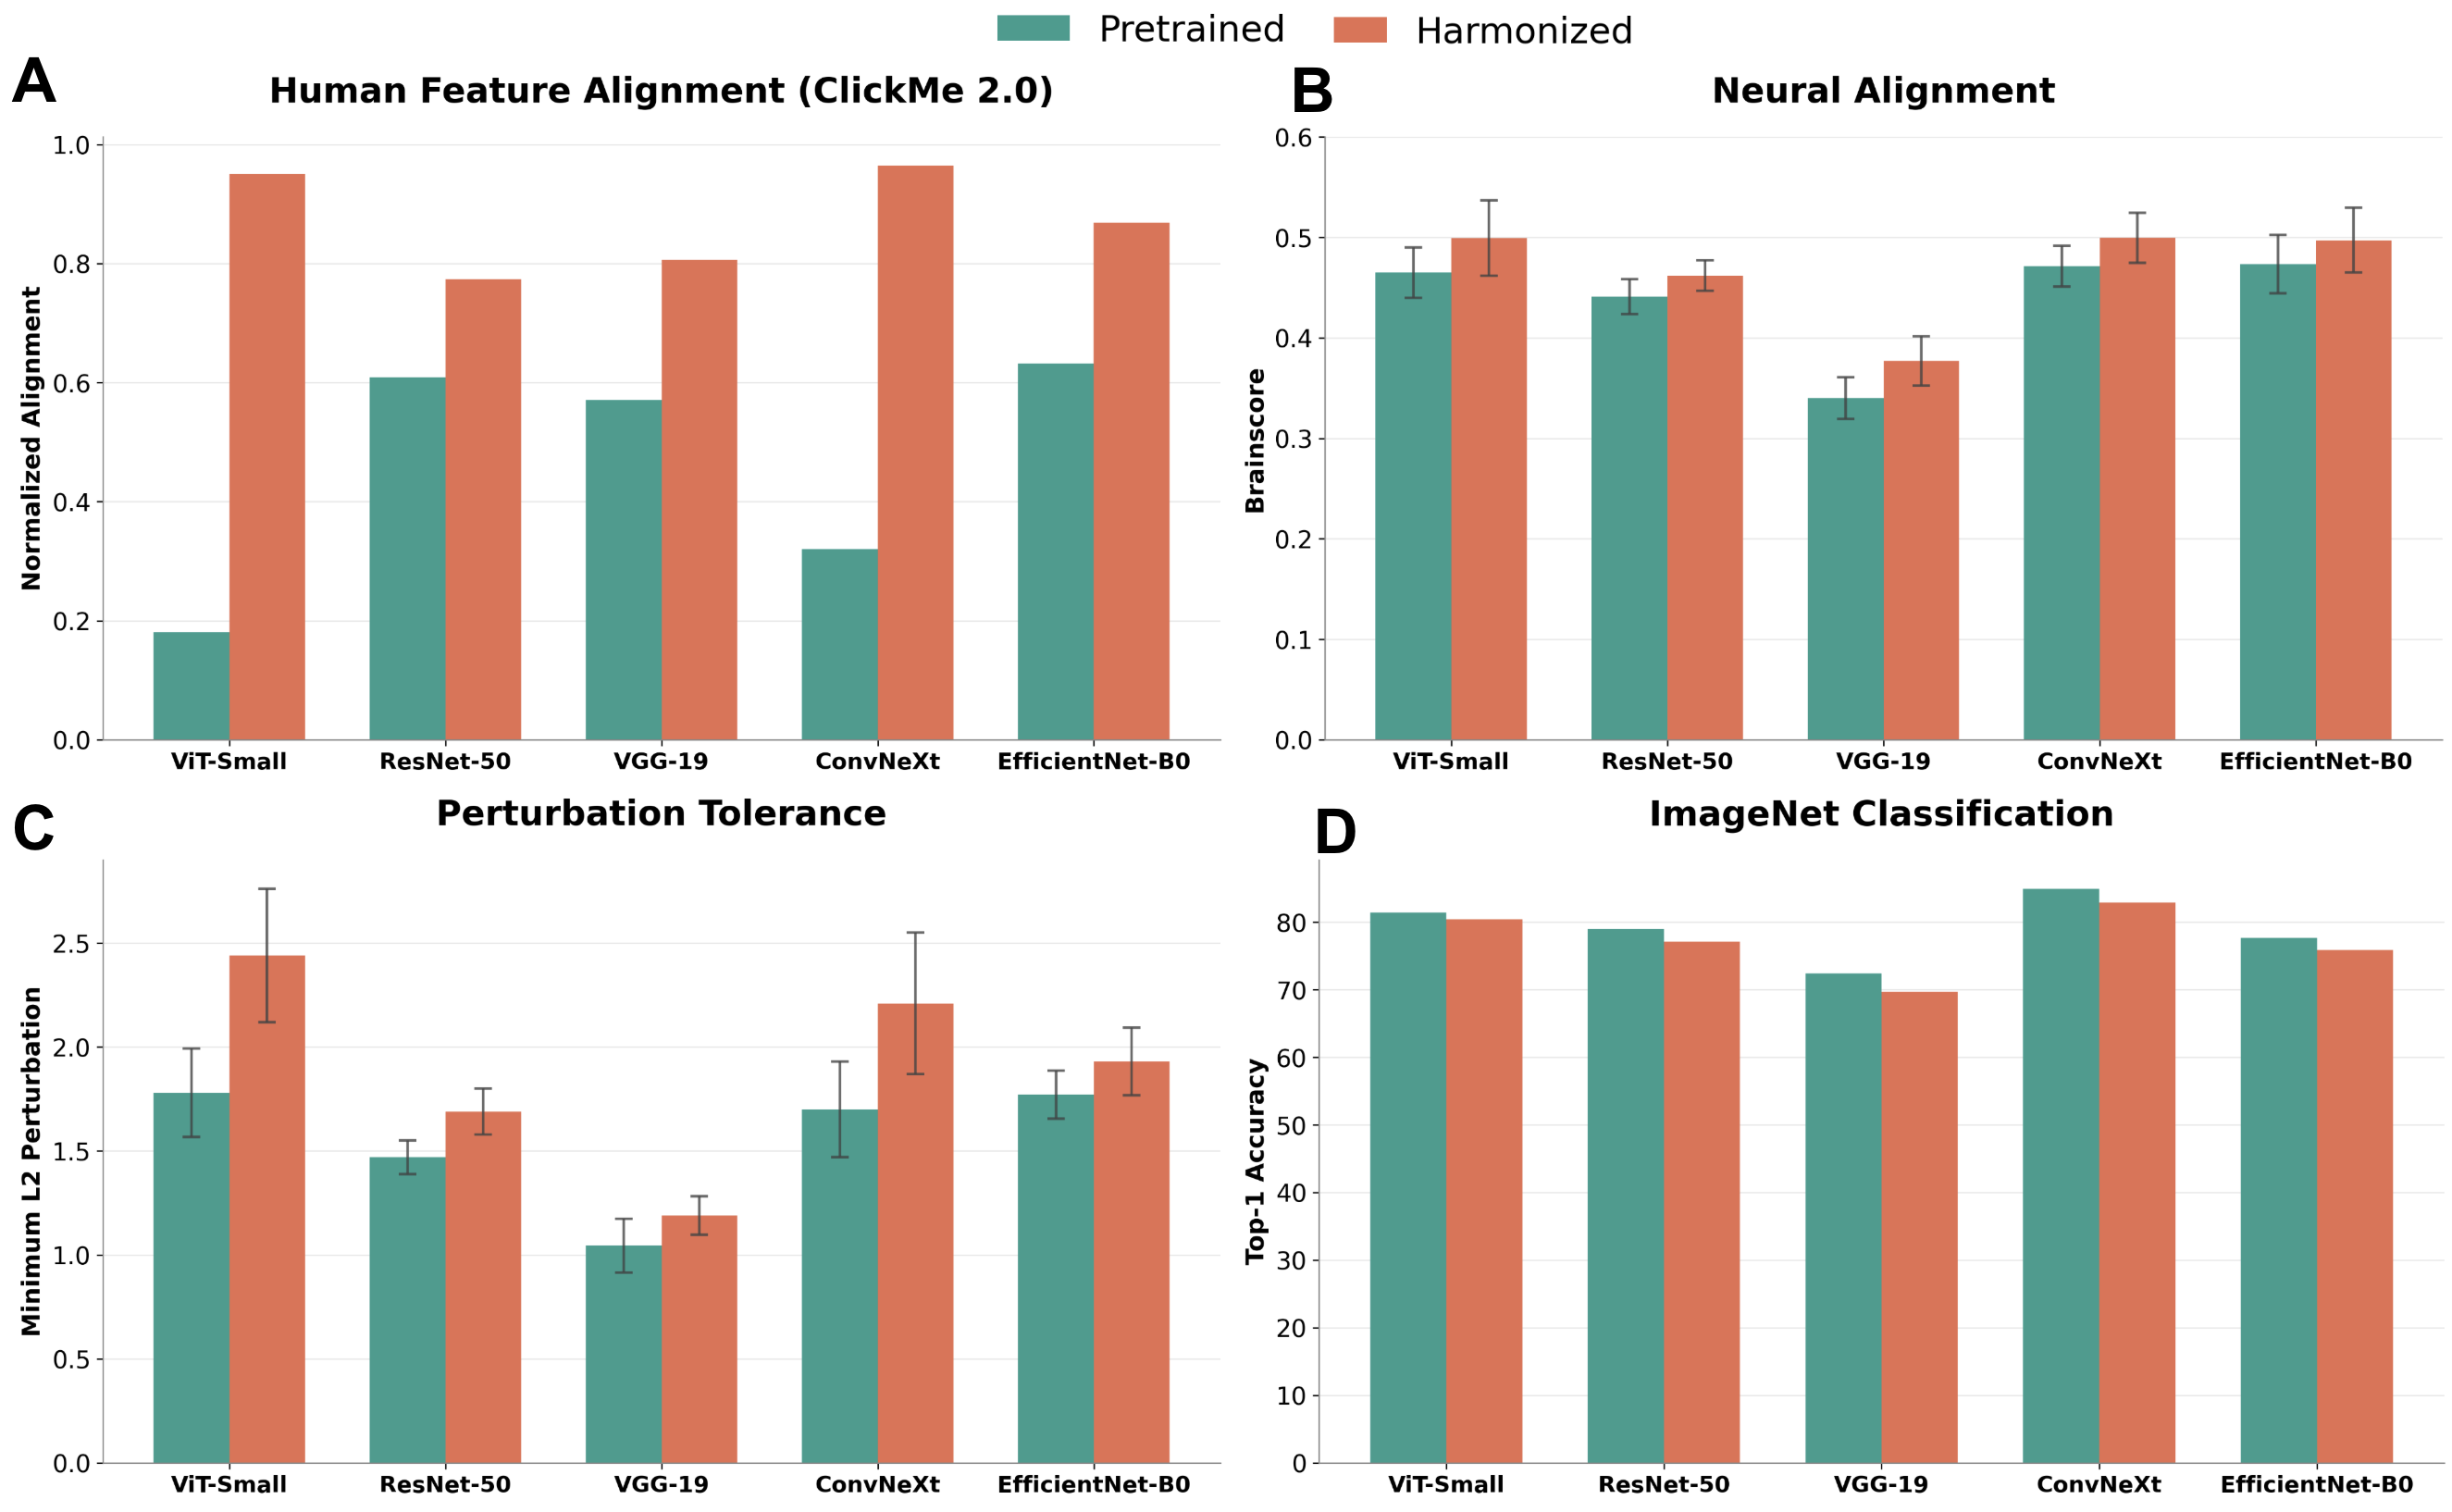
\includegraphics[width=\textwidth]{figure1.png}}{%
    \fbox{\parbox[c][2.2in][c]{\dimexpr\textwidth-2\fboxsep-2\fboxrule\relax}{%
      \centering\small\textit{Placeholder: add \texttt{figure1.png} beside the \texttt{.tex} file.}}}%
  }%
  \caption{\TS{Placeholder figure---final results pending.} A)~Neural alignment (Brain Score) on the Arcaro dataset. B)~ImageNet-1K top-1 accuracy. C)~Perturbation tolerance to L2-PGD attacks. D)~ClickMe~2.0 alignment.}
  \label{fig:results}
\end{figure*}

% \subsection{1. Reversing the Alignment Degradation in Modern Architectures}
% To evaluate the success of our psychophysical co-optimization, we first measured the spatial feature alignment of our harmonized Neural TIMM models against standard TIMM baselines using the ClickMe 2.0 dataset (Figure 1D). Standard pretrained models exhibited a concerning representational mismatch, particularly in modern, highly scaled architectures: standard \texttt{vit\_small\_patch16\_224} and \texttt{convnext} demonstrated remarkably low alignment scores (0.14 and 0.24, respectively). Following our harmonization process, we observed substantial increases across all evaluated architectures. Most notably, the architectures that diverged most from human attention under standard training paradigms saw the most dramatic improvements, with ViT and ConvNeXt alignment jumping to 0.68 and 0.59.
\paragraph{Human alignment.}
Standard TIMM models exhibit poor alignment with human visual strategies, particularly at larger scales: \texttt{vit\_small\_patch16\_224} and \texttt{convnext} score just 0.14 and 0.24, respectively, on ClickMe~2.0 (Fig.~\ref{fig:results}D). Harmonization produces large gains across all architectures, with the most misaligned models improving the most---ViT alignment rises to 0.68, ConvNeXt to 0.59.

% \subsection{2. Generalization to Physiological Brain Activity}
% Crucial to our hypothesis is that behavioral alignment organically translates to physiological alignment. We evaluated this by measuring the Neural Alignment (Brain Score) on the Arcaro fMRI dataset (Figure 1A). Across all five architectures—ranging from traditional CNNs (\texttt{vgg19}, \texttt{resnet50}) to modern transformers and hybrid models—the harmonized models consistently outperformed standard baselines. For instance, the harmonized \texttt{vit\_small} model's brain score increased from 0.60 to 0.65. This demonstrates that explicitly co-optimizing for human visual attention yields feature spaces that more closely mirror actual biological neural representations.
\paragraph{Neural predictivity.}
Harmonized models outperform TIMM baselines on the Arcaro dataset (Fig.~\ref{fig:results}A) for both CNNs (\texttt{vgg19}, \texttt{resnet50}) and transformers. For example, brain score for harmonized \texttt{vit\_small} rises from 0.60 to 0.65. Co-optimizing for human visual strategies yields representations closer to activity measured in primate visual cortex.

% \subsection{3. Biological Grounding Translates to Tangible Robustness}
% We next evaluated whether this improved biological grounding offers computational benefits, specifically regarding model robustness against visual perturbations. Figure 1C illustrates the tolerance of select architectures to L2-PGD adversarial attacks. The harmonized models exhibited markedly superior robustness compared to their standard counterparts. The harmonized \texttt{convnext} model, for example, improved its perturbation tolerance from 1.70 to 2.51. This suggests that by relying on human-like visual strategies rather than dataset-specific shortcut features, Neural TIMM models become significantly more resilient to visual distortions.
\paragraph{Robustness.}
Harmonized models are more robust to adversarial perturbations (Fig.~\ref{fig:results}C). For instance, \texttt{convnext} perturbation tolerance under L2-PGD attacks improves from 1.70 to 2.51. By relying on human-like features rather than dataset-specific shortcuts, harmonized models become substantially more resilient to visual distortions.

% \subsection{4. Performance vs. Biological Alignment Trade-offs}
% Finally, we assessed standard ImageNet1K Top-1 accuracy (Figure 1B). As expected, when actively mitigating shortcut learning and spurious correlations, we observed a minor, consistent degradation in pure benchmark accuracy across all harmonized models (e.g., standard \texttt{resnet50} accuracy shifted from 79.05\% to 77.06\% upon harmonization). Rather than a detrimental outcome, this minor trade-off is indicative of the models abandoning highly performant but brittle dataset-specific biases. By exchanging these spurious correlations for a robust and biologically plausible feature space, Neural TIMM provides a substantially more predictable starting point for transfer learning.
\paragraph{Accuracy trade-off.}
Harmonization produces a small, consistent decrease in ImageNet top-1 accuracy (e.g., \texttt{resnet50} drops from 79.05\% to 77.06\%; Fig.~\ref{fig:results}B). This is expected: the models are abandoning brittle shortcut features in favor of a more robust, biologically grounded feature space.

\section{Discussion}

These results show that harmonization scales effectively across a diverse set of architectures when combined with ClickMe~2.0 and efficient fine-tuning. The generalization from behavioral alignment to neural predictivity in macaque cortex reinforces the view that human perceptual strategies reflect something fundamental about biological visual processing \citep{LinsleyFengSerreTICS}. We release all harmonized weights as an open resource, providing the community with pretrained models that are both performant and meaningfully aligned with biological vision.

\printbibliography

\end{document}
